\documentclass[11pt,a4paper]{article}
\usepackage[utf8]{inputenc}
\usepackage[francais]{babel}
\usepackage[T1]{fontenc}
\usepackage{amsmath}
\usepackage{amsfonts}
\usepackage{amssymb}
\usepackage{graphicx}
\usepackage{caption}
\usepackage[left=2cm,right=2cm,top=2cm,bottom=2cm]{geometry}
\author{Bastien Duraj - Carreteros Laetitia - Gentile Pierre - Didier--Roche François}
\title{Rapport intermédiaire du projet de développement web 2}


\begin{document}

\maketitle
\newpage

\tableofcontents
\newpage

\section{Description de l'application}
Pour ce projet de développement web nous avons choisi de faire une application permettant de créer de manière collaborative une \textbf{carte mentale}. Elles seront composées de nœuds reliés entre eux et il existera une hiérarchisation entre ceux-ci (un nœud est fils d'un autre, ...). Il y aura également la possibilité de mettre du texte dans un nœud pour représenter l'idée associée à celui-ci. 
En ce qui concerne le document qui sera partagé sur le serveur il s'agira directement d'un fichier XML permettant de représenter de l'information de manière hiérarchisée et donc parfaitement adapté à notre type de document. 

Pour finir avec la description globale de notre application voici une
liste des différentes fonctionnalités que nous avons mise en place :
\begin{itemize}
\item Pour le client lourd et léger:
	\begin{enumerate}
     	\item Intégration d'un chat interne à l'application.
     	\item Possibilité de se connecter à son compte.
     	\item Possibilité de gérer son compte.
     	\item Possibilité de créer des document.
     	\item Possibilité de zoomer ou dézoomer le graphe.
	\end{enumerate}
\item Pour les nœuds:
	\begin{enumerate}
     	\item Modification des nœuds : nom, dimensions.
     	\item Ajout, suppression et déplacement d'un nœud.
     	\item Possibilité de décrire un nœud pour préciser sa fonction.
	\end{enumerate}
\item Pour la communauté:
	\begin{enumerate}
     	\item Possibilité de discuter les membre du groupe associés a
          un document.
     	\item Possibilité de créer des groupes.
	\end{enumerate}
\end{itemize}
Dans la suite de ce rapport, nous verrons dans un premier temps les
différents shémats que nous avons utilisée comme ligne directrice tout
au long de notre projet.

\section{Diagrammes}
Pour notre application nous avons également crée 4 types de diagrammes UML (Classe, BDD, Cas d'utilisation et Séquence) avec un schéma entité-association.\\
\textbf{Remarque: Tous les diagrammes présentés ne sont pas définitif et sujet à modification. De plus une version en grand format de chacun des diagrammes est fournit en Annexe à la fin de ce rapport.}
\subsection{Schéma entité-association}
Ce schéma représente les relations entre les différents objets de notre application, il s'agit du premier schéma que nous avons établi ce qui a permis par la suite de mettre en place une base de données claire et complète.
\begin{figure}[!h]
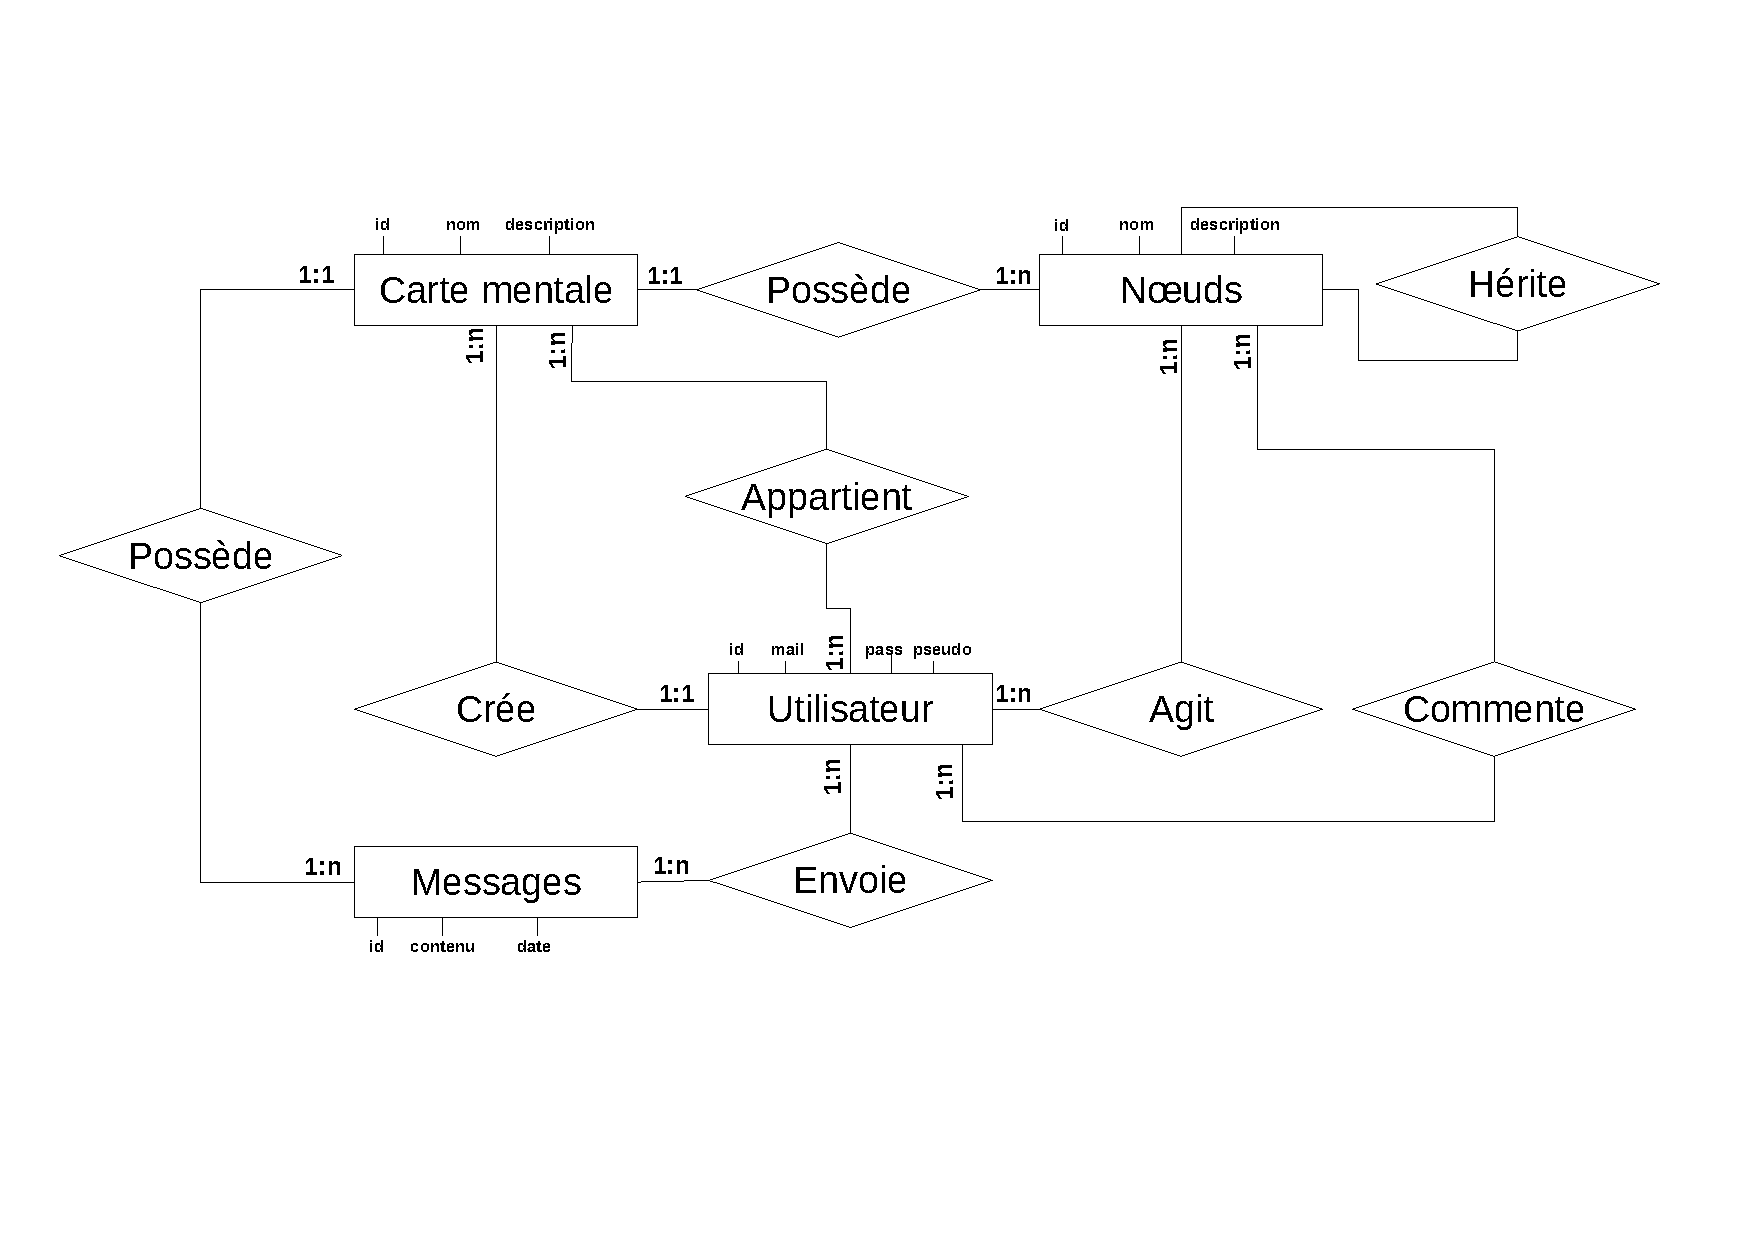
\includegraphics[scale=0.5]{Image/Schema_entite_association.pdf}
\caption{Schéma entité-association de l'application}
\end{figure}
\subsection{Diagramme des tables de la BDD}
La base de donnée représenté ici nous permettra de stocker les différentes informations relative à un utilisateur ou à un groupe de travail avec les messages envoyés entre les différents utilisateurs.
\begin{figure}[!h]
\centering
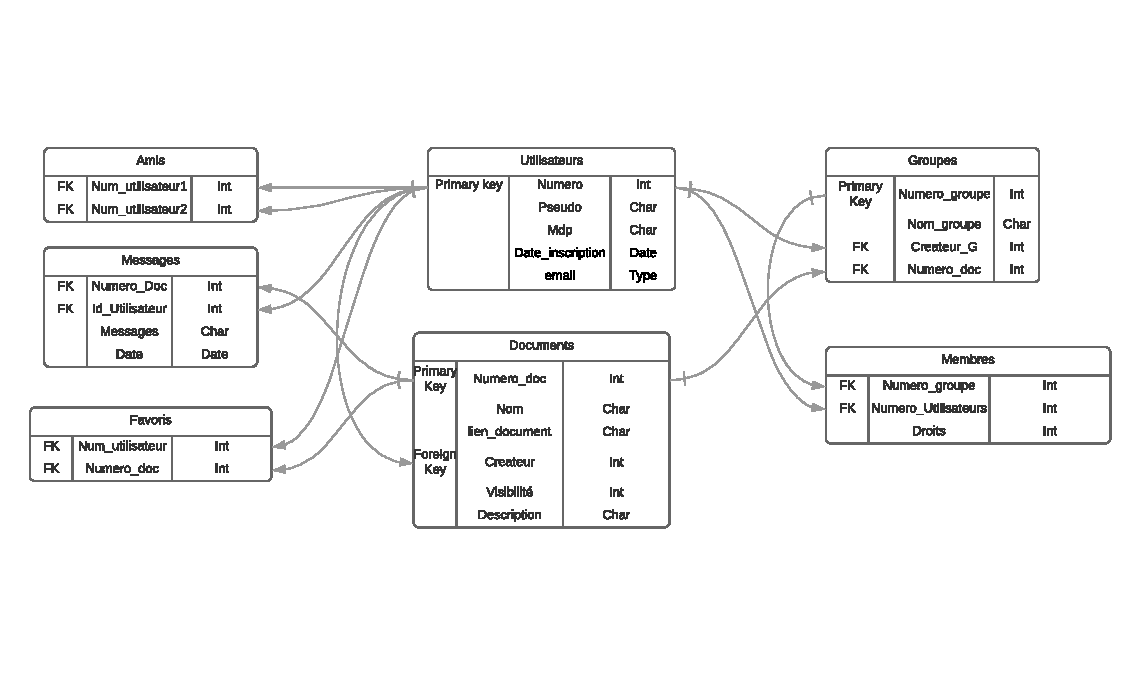
\includegraphics[scale=0.6]{Image/Diagramme_BDD.pdf}
\caption{Tables et relation entre les données de la BDD}
\end{figure}
\subsection{Diagramme des cas d'utilisation}
Ce schéma est une représentation simple et claire des différentes possibilités auxquelles un type d'utilisateur peut accéder. Nous avons dans ce schéma 'hiérarchisé' les différents acteurs suivant leur importance dans le document, le chef de groupe étant au-dessus (en terme de choix d'action) des autres acteurs. \\
\textbf{Remarque: Dans un souci de lisibilité des flèches n'ont pas été montré, le chef du groupe peut très bien faire les actions d'un membre du groupe ou d'un spectateur, ect... .}
\begin{figure}[!h]
\centering
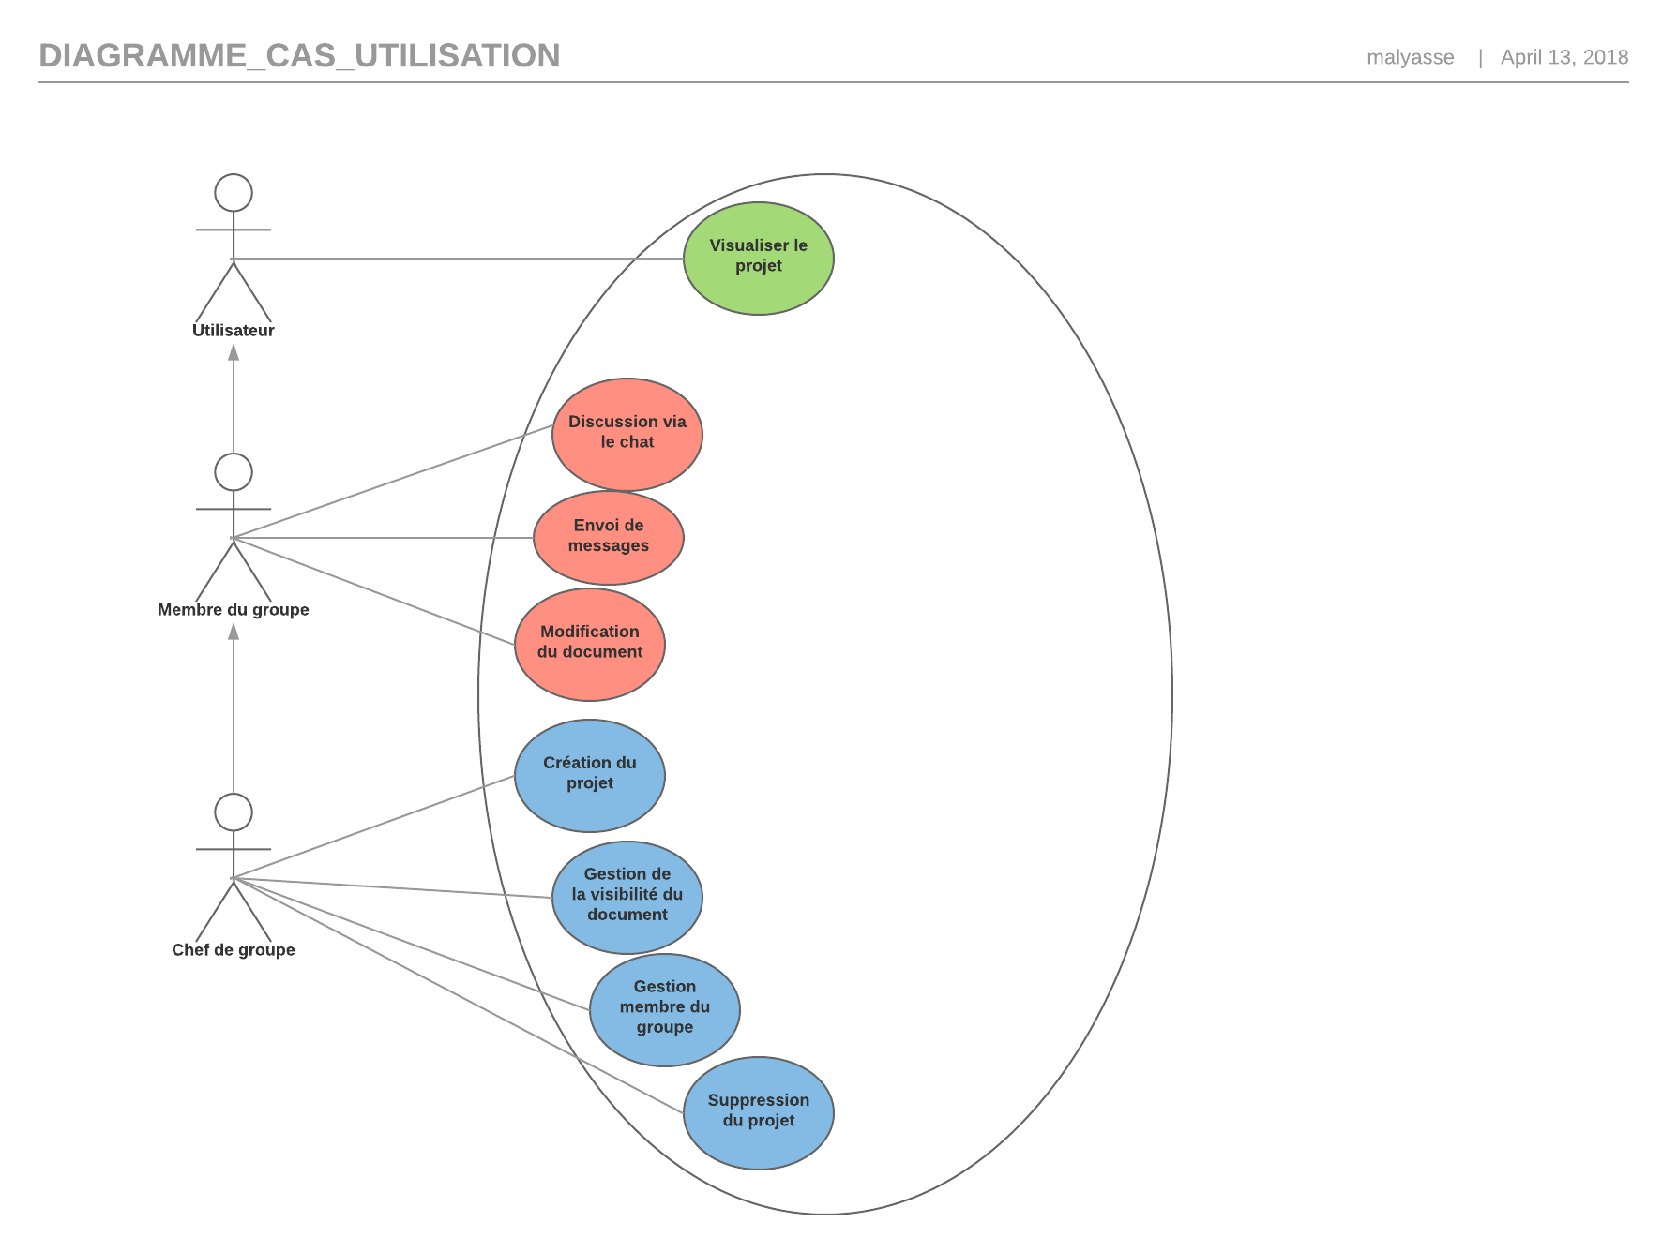
\includegraphics[scale=0.5]{Image/Diagramme_cas_utilisation.pdf}
\caption{Représente les différentes actions possibles pour chaque type d'utilisateur}
\end{figure}
\subsection{Diagramme de séquence}
Nous avons divisé notre diagramme de séquence en 3 parties, un par scénario, où nous mettons en scène à chaque fois un type d'utilisateur: le créateur du document, un membre du groupe de travail et un simple spectateur.
\subsubsection{Scénario 1}
Le premier scénario met en scène l'utilisateur créant un document, on y voit les interactions entre le serveur, le client et la base de données.
\newpage
\begin{figure}[!h]
\centering
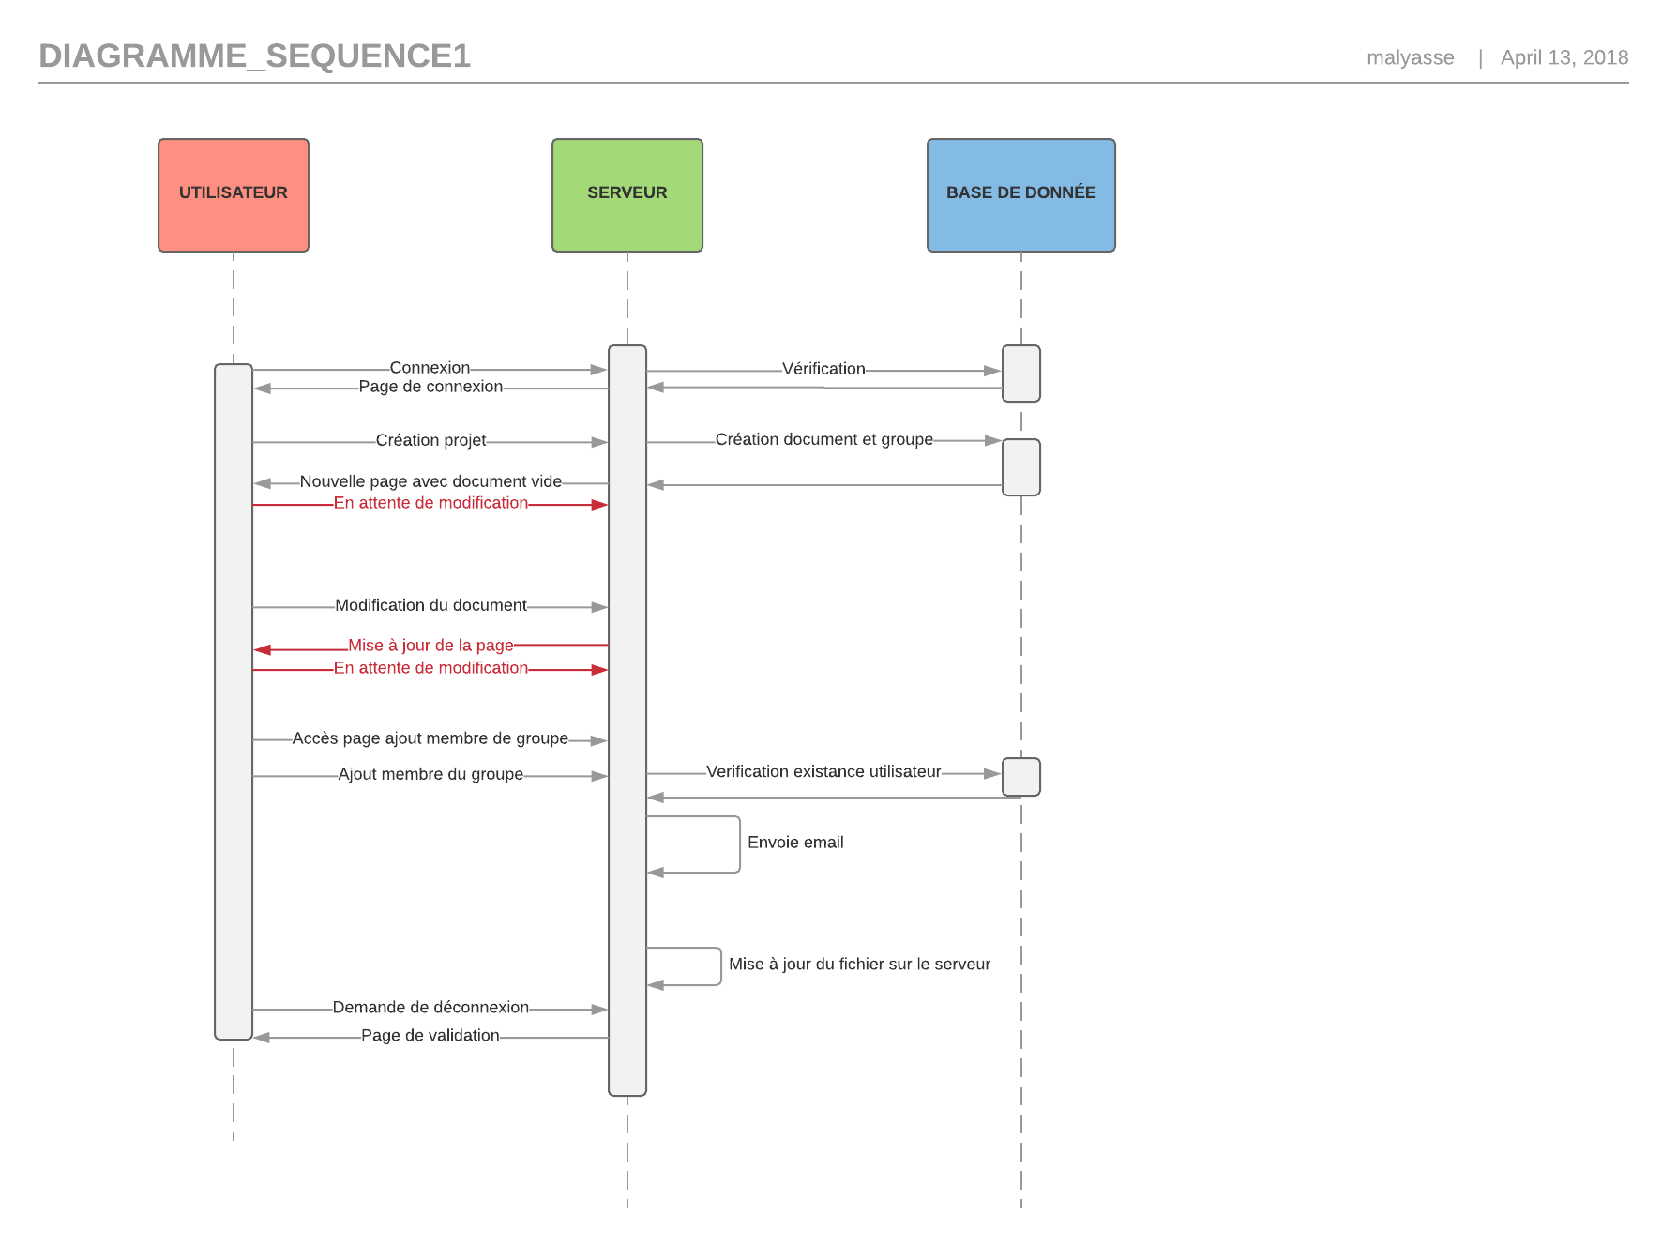
\includegraphics[scale=0.5]{Image/Diagramme_sequence1.pdf}
\caption{Représente le déroulement d'un scénario entre trois acteurs: Utilisateur, serveur, BDD}
\end{figure}
\subsubsection{Scénario 2}
Dans ce scénario on retrouve 2 utilisateurs qui discutent via le 'tchatche' interne à l'application et unique à chaque projet, et via la messagerie qui concerne toute l'application.
%\begin{figure}[!h]
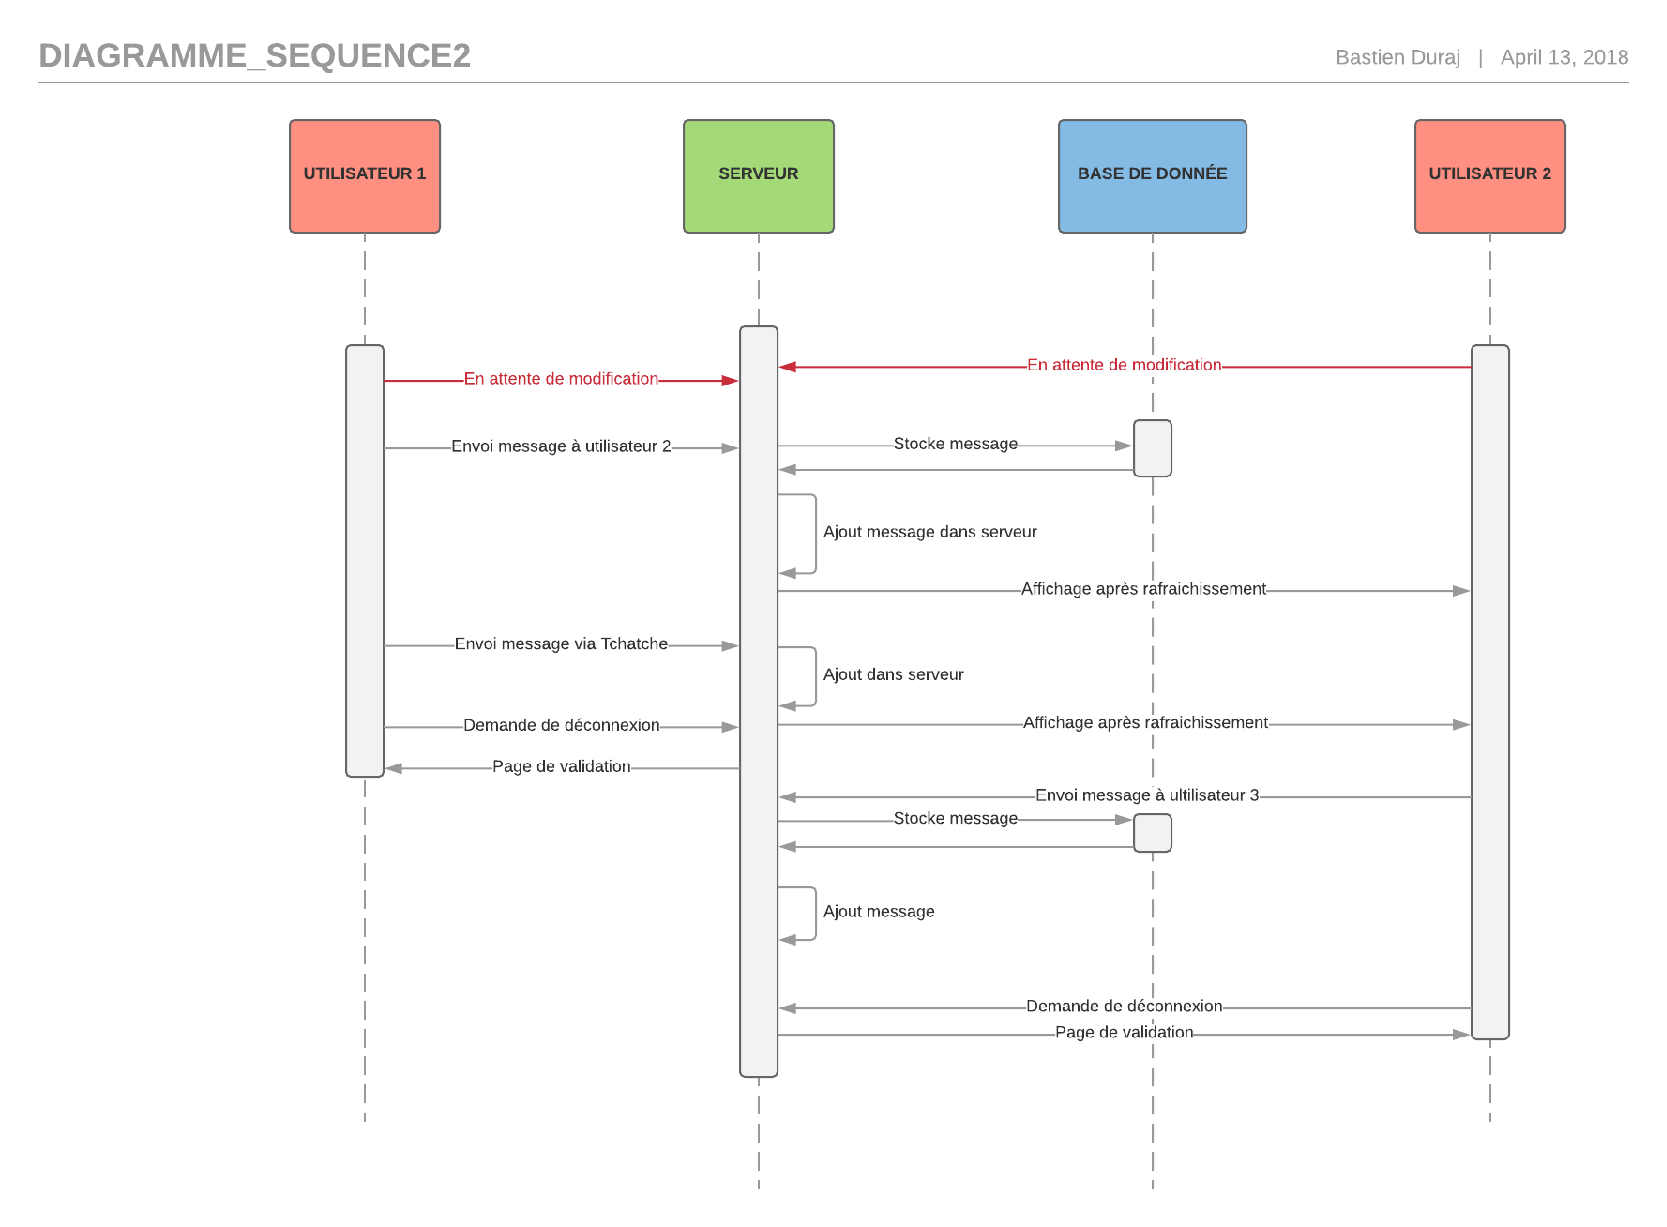
\includegraphics[scale=0.5]{Image/Diagramme_sequence2.pdf}
\captionof{figure}{Représente le déroulement d'un scénario entre quatre acteurs: Utilisateur, serveur, BDD et un autre utilisateur}
%\caption{Représente le déroulement d'un scénario entre quatre acteurs: Utilisateur, serveur, BDD et un autre utilisateur}
%\end{figure}

\subsubsection{Scénario 3}
Le troisième scénario met en scène un spectateur qui fait une demande d'inscription puis demande la visualisation d'un document.
\begin{figure}[!h]
\centering
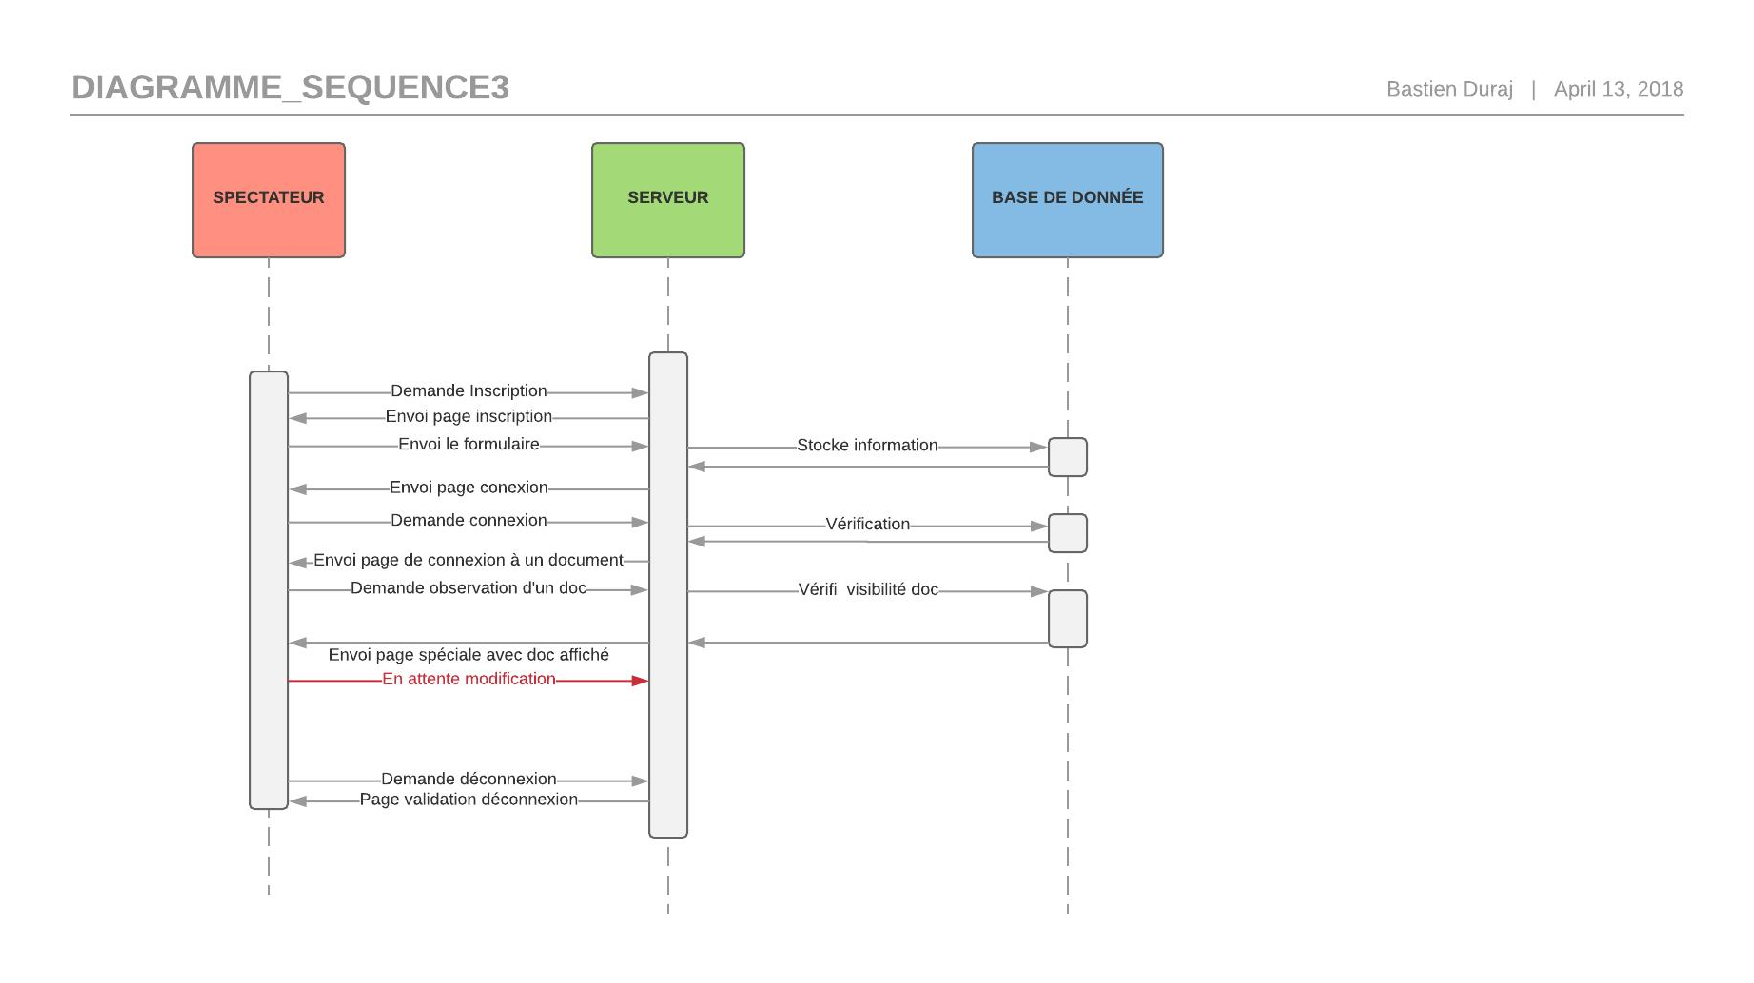
\includegraphics[scale=0.5]{Image/Diagramme_sequence3.pdf}
\caption{Représente le déroulement d'un scénario entre trois acteurs: Spectateur, serveur, BDD}
\end{figure}

\subsection{Diagramme des classes}
Pour finir nous présentons ici \textbf{un premier jet} de notre diagramme des classes.
\begin{figure}[!h]
\centering
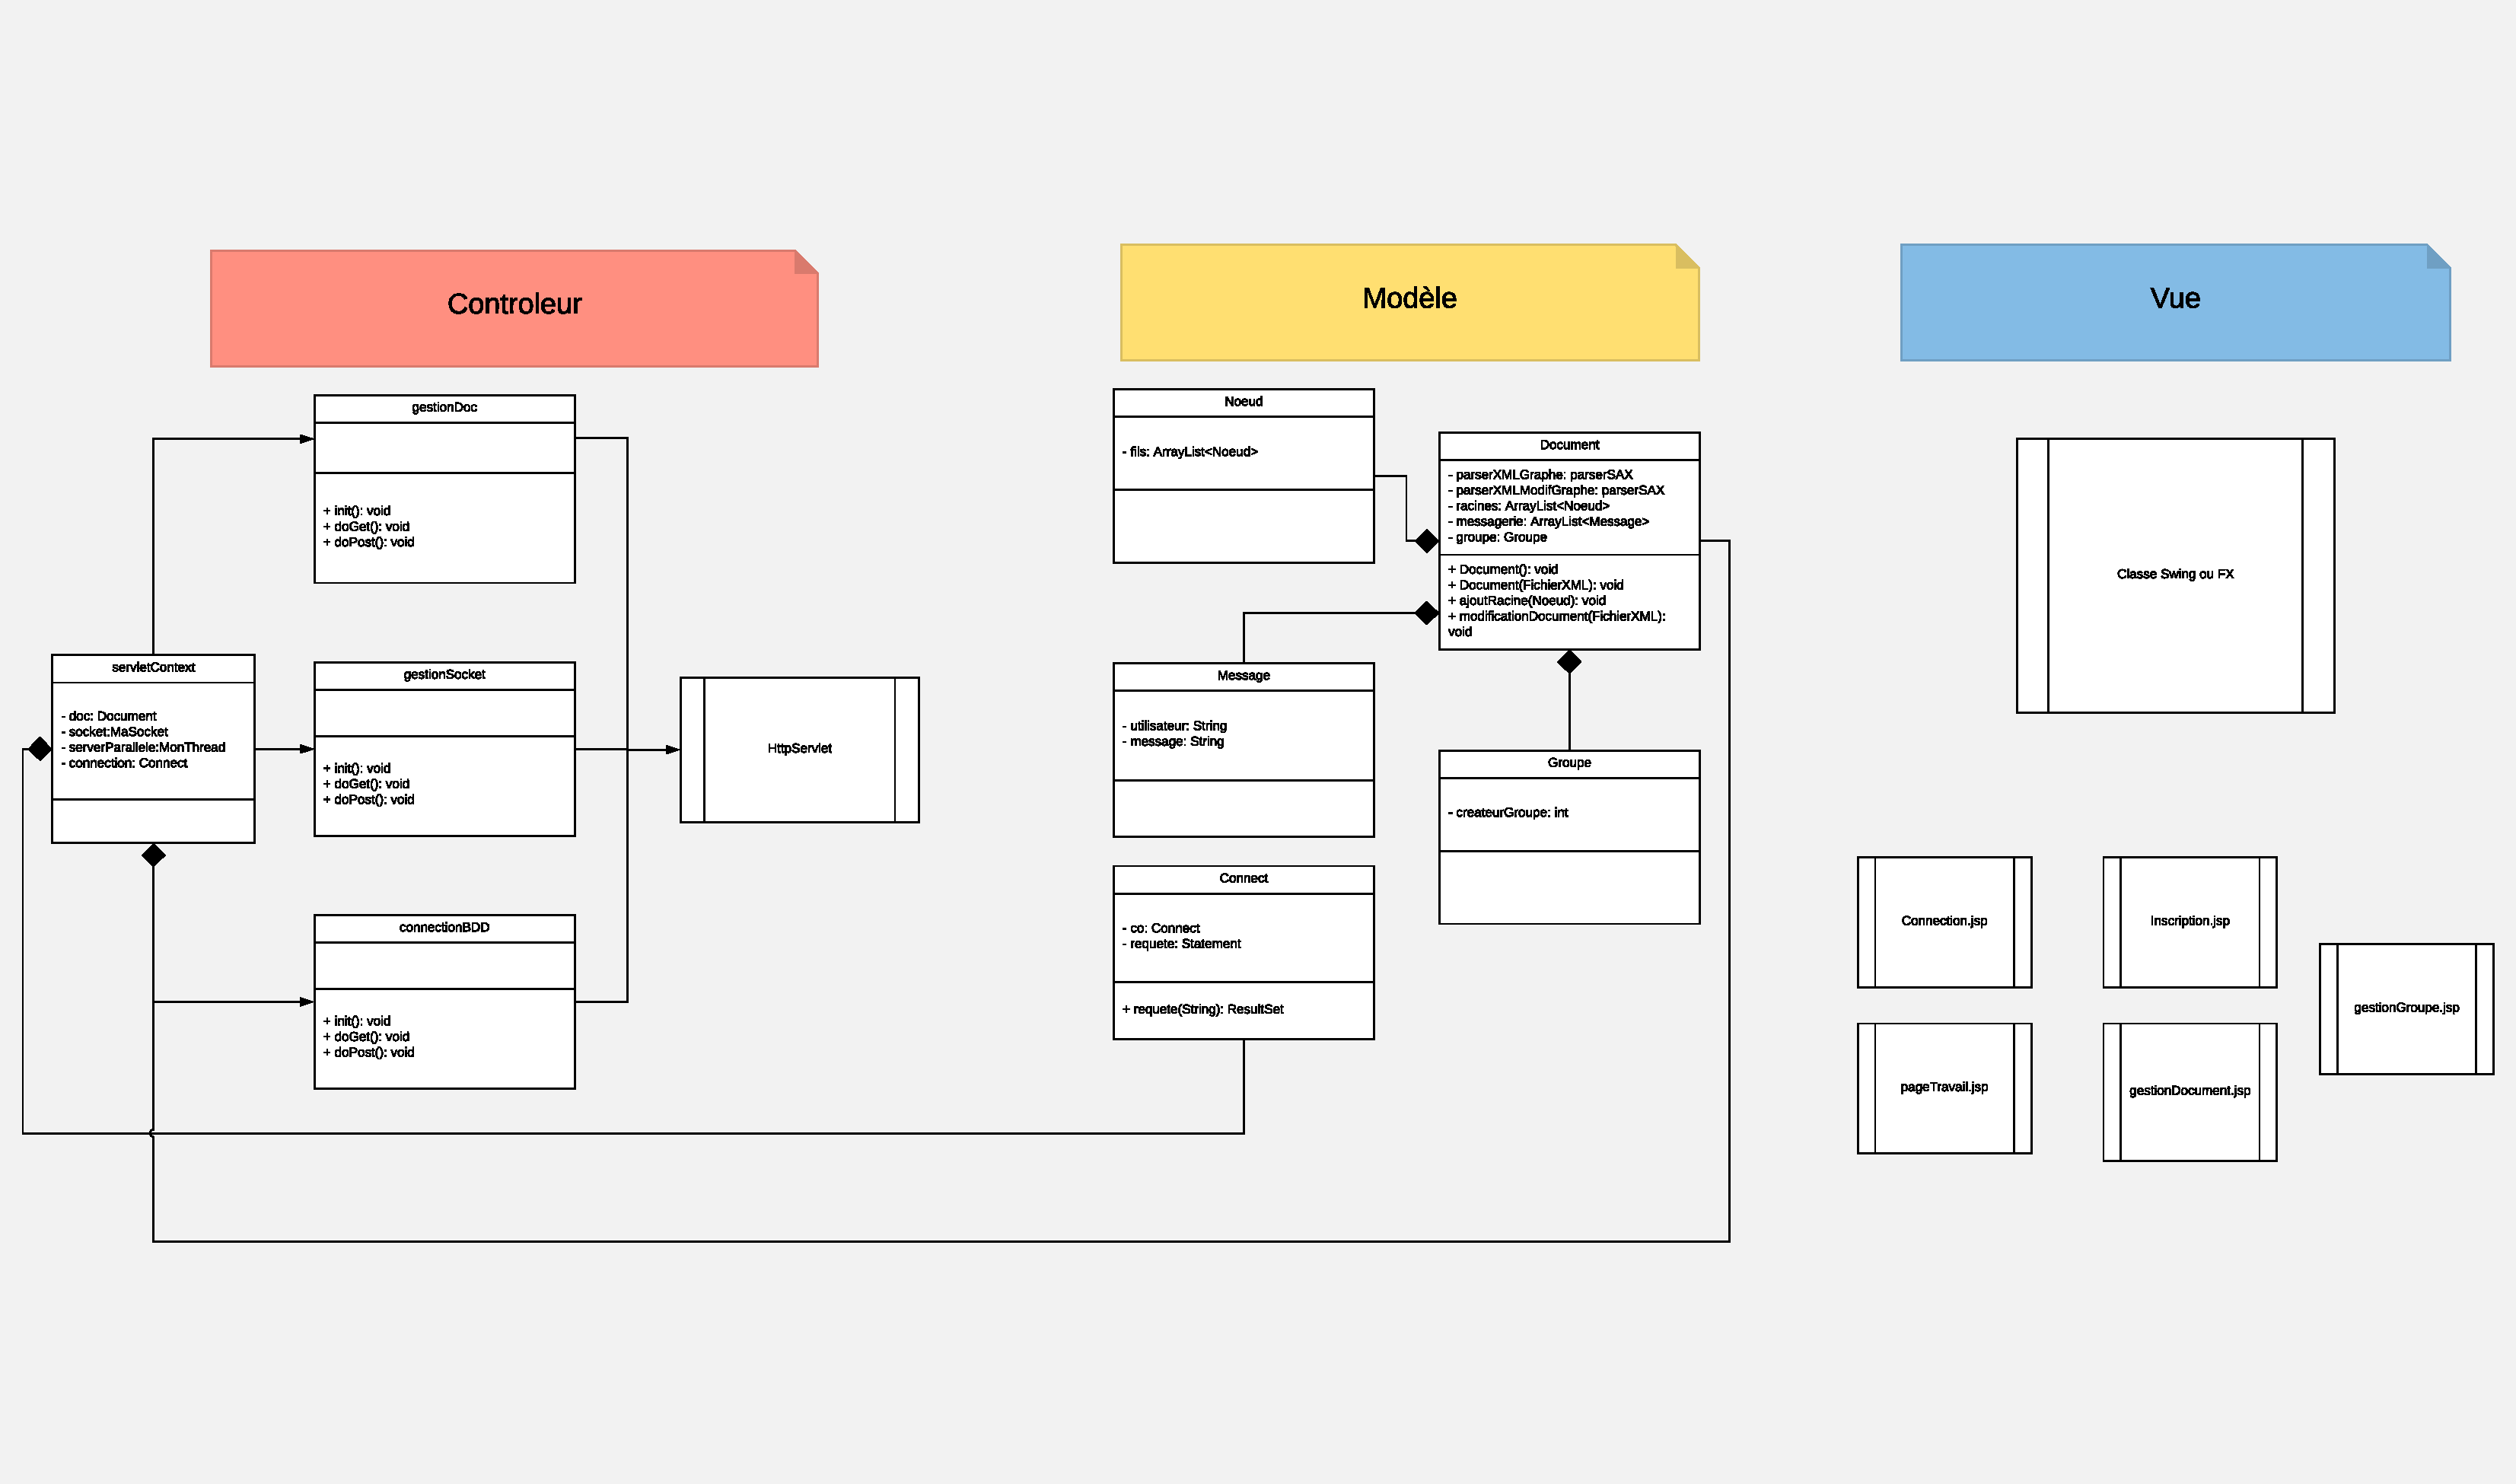
\includegraphics[angle=0, scale=0.3]{Image/Class_Diagram_dev2.pdf}
\caption{Diagramme des classes de notre application divisé en 3 parties suivant l'architecture MVC pour plus de visibilité}
\end{figure}
\section{Application des technologies}
Avant de passer à la distribution du travail entre les différents membres de notre groupe nous allons revenir de manière plus précise sur l'utilisation des différentes technologies dans notre application.
\subsection{Client Léger}
\paragraph{•}
\textbf{Utilisation des Servlets}\\
Elles permettent de contrôler les accès aux données qu'ils s'agissent de la BDD ou des données représentées en mémoire comme notre document. Lorsqu'un client envoie une requête faisant intervenir ces données, la servlet interne à la JSP fait appel à une servlet spéciale faisant office de contrôleur. Une servlet spéciale servira également à gérer la socket (récupération des données) permettant de faire le lien entre la partie serveur et le client lourd.

\paragraph{•}
\textbf{Utilisation des JSPs}\\
Les JSP dans notre application servent à représenter les différentes pages du client léger mais également à communiquer avec les contrôleurs. Elles communiqueront avec le serveur grâce à des formulaires.

\paragraph{•}
\textbf{Utilisation de la librairie JDBC}\\
Elle nous permet de créer une communication entre le serveur et la base de données et de soumettre nos différentes requêtes.

\subsection{Client Lourd}
\paragraph{•}
\textbf{Utilisation de la librairie JDBC}\\
Elle nous permet de créer une communication entre le serveur et la base de données et de soumettre nos différentes requêtes.
\paragraph{•}
\textbf{Utilisation des fichiers XML}\\
Les fichiers XML servent à représenter notre graphe pour et de pouvoir
le modifier grâce a un parseur DOM.

\paragraph{•}
\textbf{Utilisation de java FX}\\
La bibliothèque Java FX nous a permis de créer les interfaces de
connexion, inscription, gestion de compte pour le client lourd. Elle
nous a aussi permis de représenter le document partagé par un fichier
XML. En effet, la représentation des vues avec JavaFX utilise des
fichiers XML representant les éléments affichés a l'écran. Dans la
zone de représentation du document, les noeuds et leurs sont donc représentés
par un fichier XML.
\paragraph{•}
\textbf{Utilisation des Sockets}\\
Les sockets nous ont permis de gérer la communication entre le client
lourd et la parti serveur. Lorsque l'utilisateur apporte certaines
modifications à un fichier XML (représentation du graphe)
l'information est transmise au serveur afin de faire les modification
sur ce graphe. Cette transmission d'information permet aussi de
verifier la connexion d'un utilisateur à partir du client lourd,
d'envoyer les données necessaires lors de l'inscription d'un
utilisateurs ou de la modification de son compte.

\section{Origine du code}
Le code est majoritairement 100\% personnel. Certaines partie du code
sont faite avec l'appuis de tutoriel. Les parties copiée telles quelles
sont indiquées dans le code source.

\section{Distribution et temps de travail}
Pour conclure ce rapport intermédiaire nous parlerons de la distribution du travail entre les différents membres du groupe:\\
\paragraph{•} Pierre Gentile a majoritairement fais la partie
JSP/Servlet et plus précisément le divers menus du client
leger. (15-25h de travail).
\paragraph{•} Bastien Duraj s'est occupé de la partie base de données
et sockets. Il a aussi developper certaines JSP et Servlets que l'on
retrouve dans le client léger.
\paragraph{•} François Didier--Roche s'est occupé de développer la
totalitée du client lourd.
\paragraph{•} Laetitia Carreteros s'est occupée de la partie mise en
forme du client leger. Elle a aussi participer au developpement du
client leger.


\textbf{Chef d'équipe:} Duraj Bastien.

\newpage

\section{Les ressouces utilisées}
\paragraph{•} Utilisation de git et github pour la gestion de sources.
\paragraph{•} Utilisation de JDBC pour la partie base de données.
\paragraph{•} Utilisation de la JSTL pour les JSP.
\paragraph{•} https://openclassrooms.com/
\paragraph{•} https://stackoverflow.com/

\section{Conclusion}
Pour conclure, nous pensons avoir été trop ambitieux sur le contenu de
l'application web. En effet, la fonctionnalitée principale, c'est à
dire la représentation du graphe à la fois sur le client lourd et le client
leger fût difficile dans sa conception. D'une part, car la communication
entre client lourd et serveur fût difficile. D'autre part car nous
n'avons pas réussi à representer le graphe sur le client leger. Nous
pensons que nous avons manquer de temps pour produire une application
totalement fonctionelle. Certaines technologies obligatoire pour faire
ce projet nous ont parru difficile. Nous Pensons ne pas avoir eu assez
d'expérience lors de ce semestre pour produire une telle application
en si peut de temps.  


\newpage
\section{Annexe}
\subsection{Schéma entité-association}
\begin{figure}[!h]
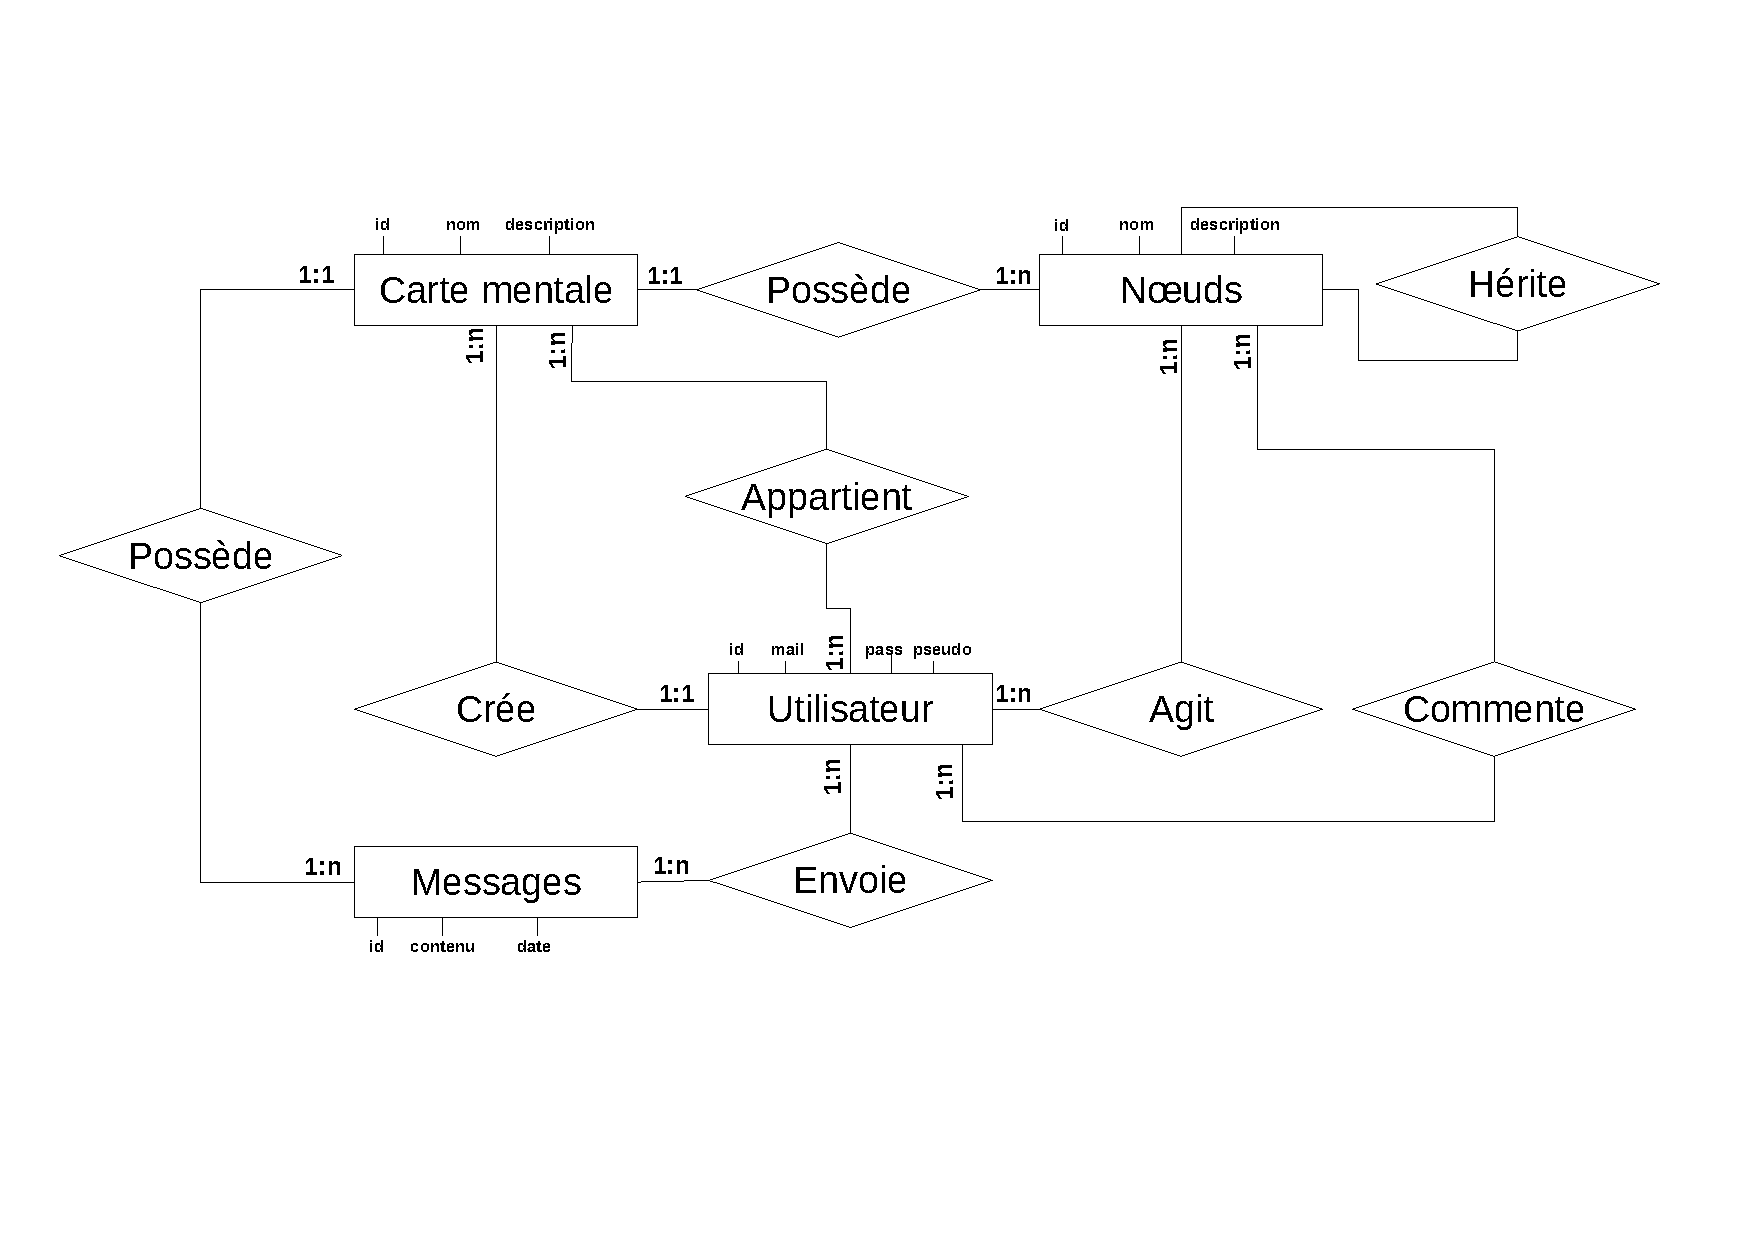
\includegraphics[angle=270, scale=0.6]{Image/Schema_entite_association.pdf}
\caption{Schéma entité-association de l'application}
\end{figure}
\newpage
\subsection{Diagramme des tables de la BDD}
\begin{figure}[!h]
\centering
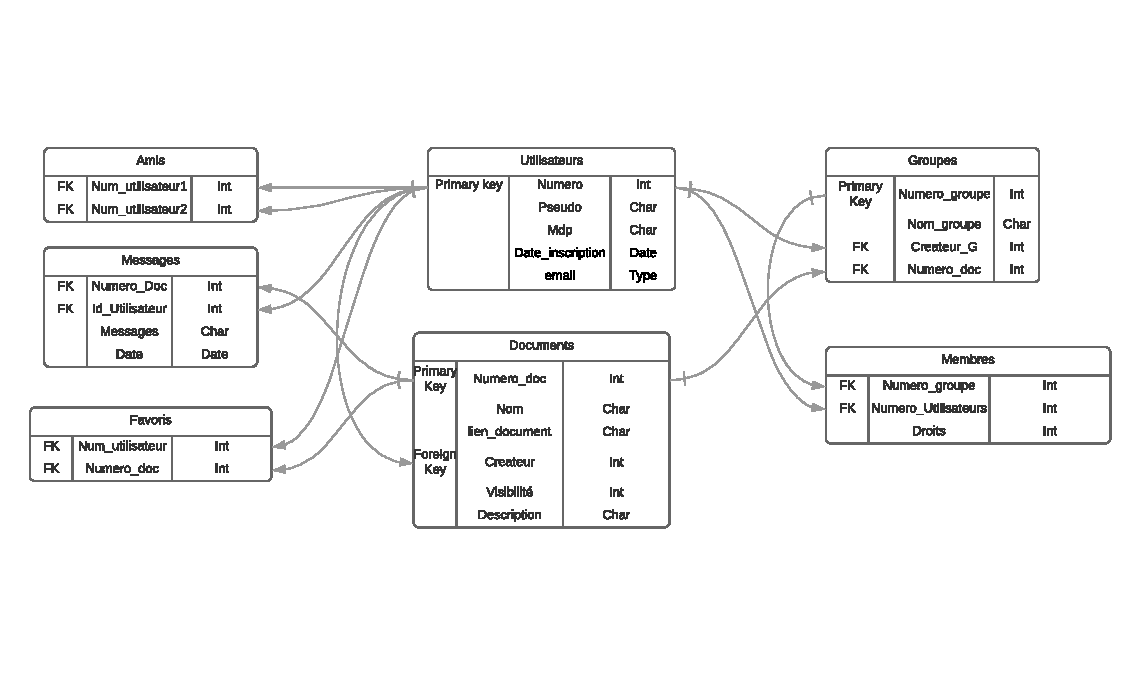
\includegraphics[angle=270, scale=0.7]{Image/Diagramme_BDD.pdf}
\caption{Tables et relation entre les données de la BDD}
\end{figure}
\newpage
\subsection{Diagramme des cas d'utilisation}
\begin{figure}[!h]
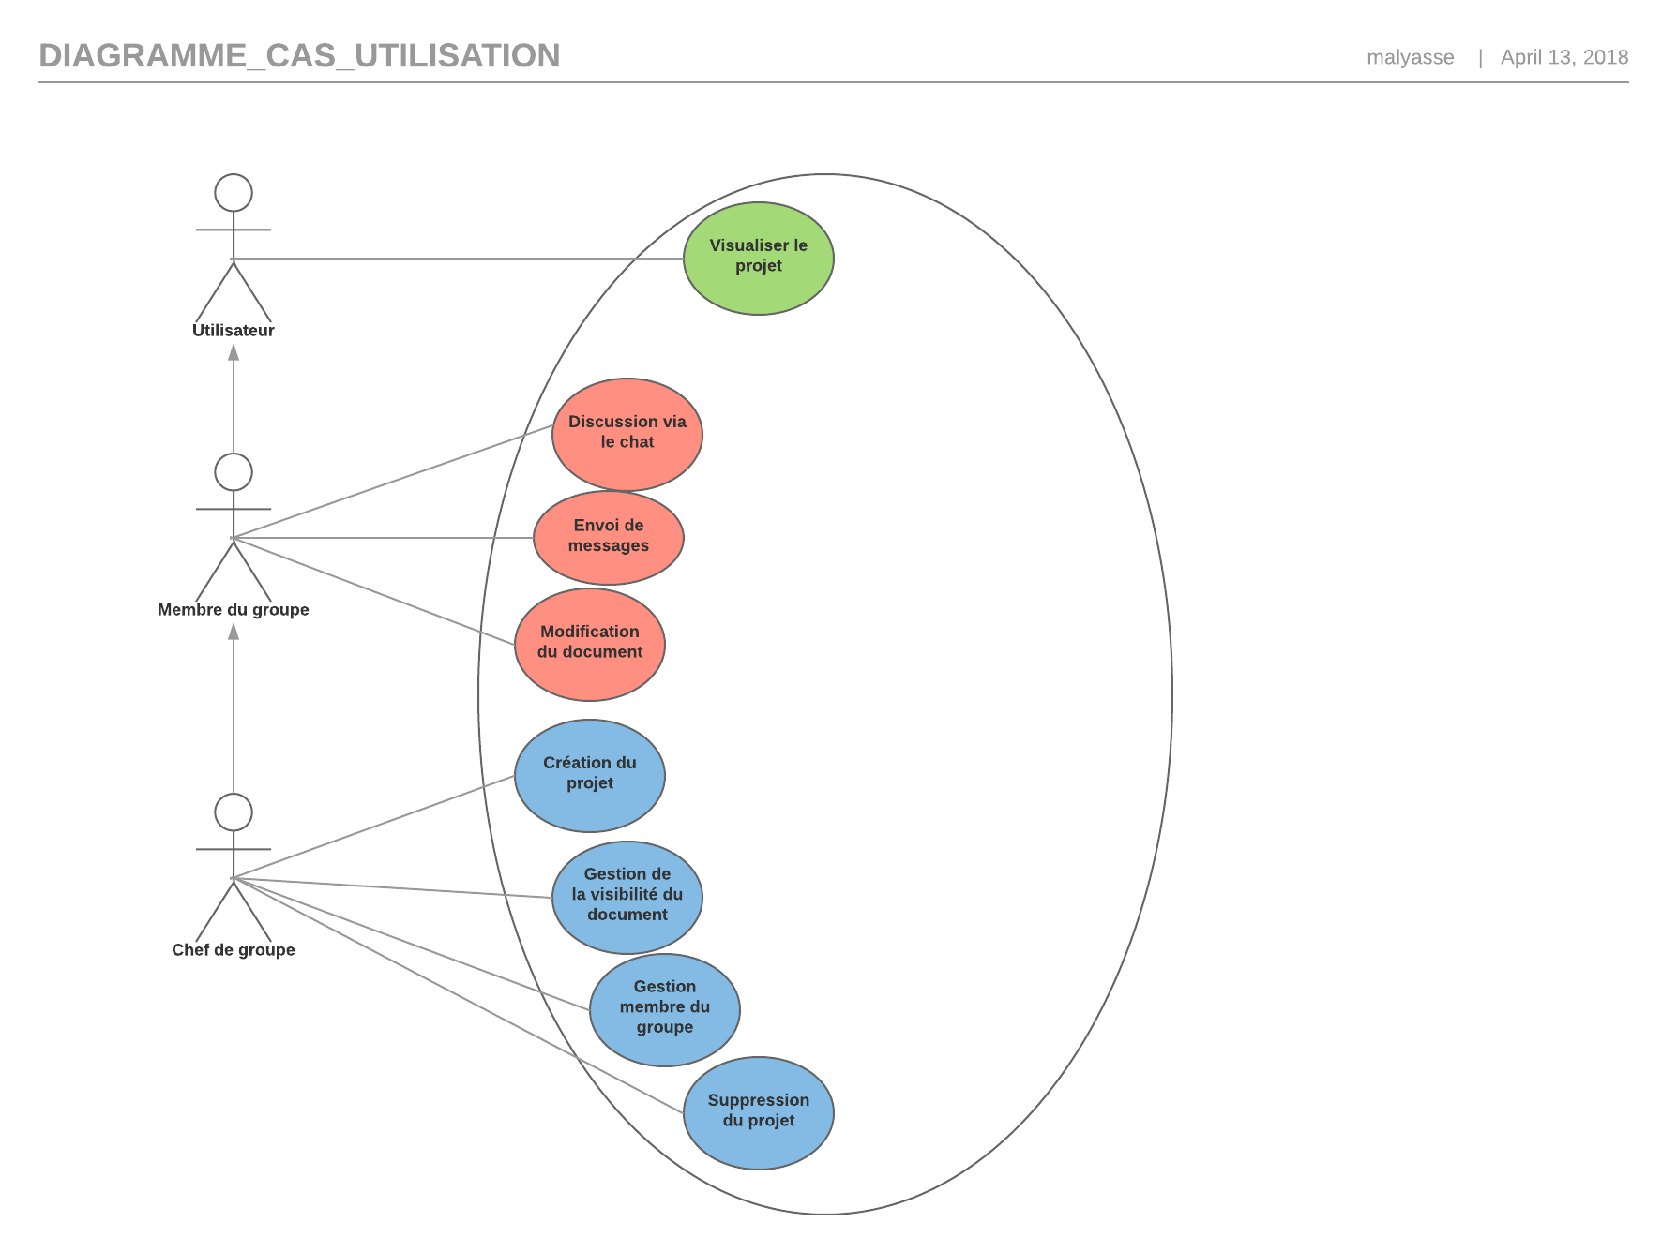
\includegraphics[scale=0.7]{Image/Diagramme_cas_utilisation.pdf}
\caption{Représente les différentes actions possibles pour chaque type d'utilisateur}
\end{figure}
\newpage
\subsection{Diagramme de séquence 1}
\begin{figure}[!h]
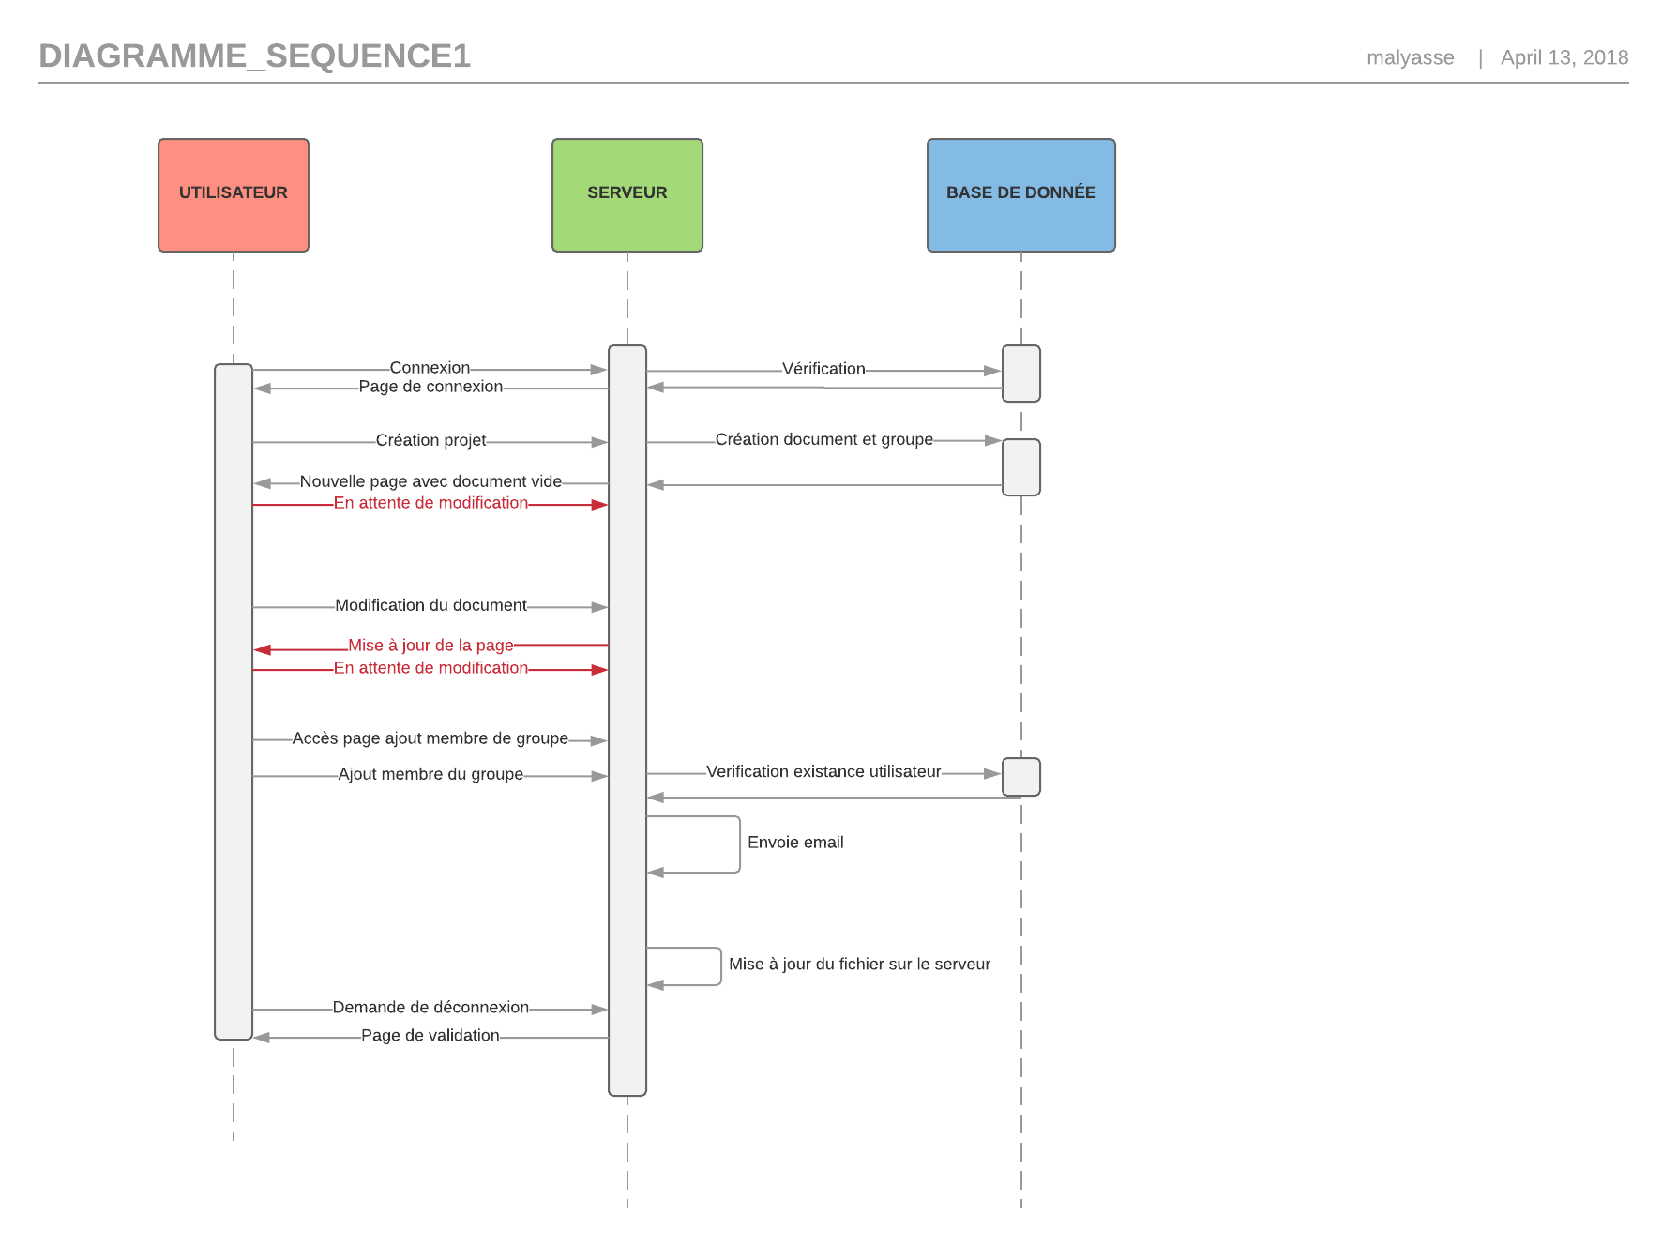
\includegraphics[scale=0.7]{Image/Diagramme_sequence1.pdf}
\caption{Représente le déroulement d'un scénario entre trois acteurs: Utilisateur, serveur, BDD}
\end{figure}
\newpage
\subsection{Diagramme de séquence 2}
\begin{figure}[!h]
\centering
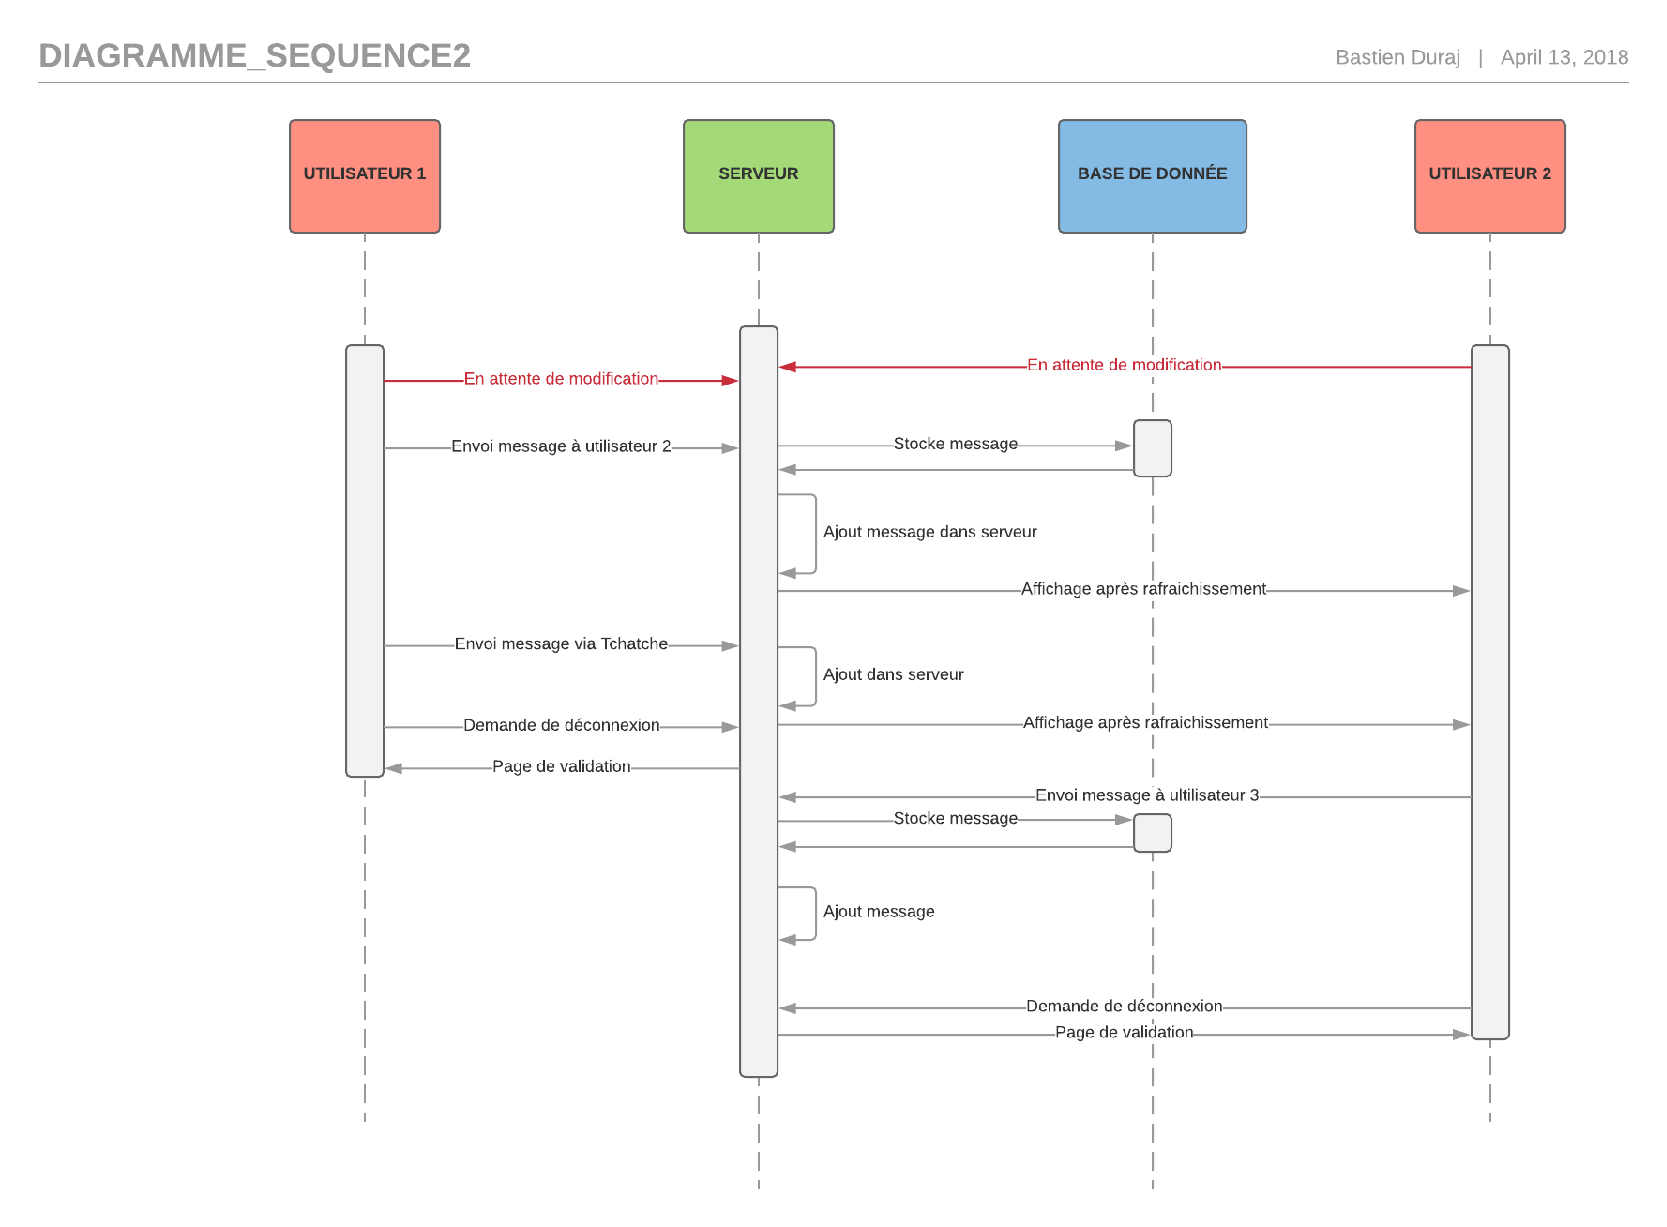
\includegraphics[scale=0.6]{Image/Diagramme_sequence2.pdf}
\caption{Représente le déroulement d'un scénario entre quatre acteurs: Utilisateur, serveur, BDD et un autre utilisateur}
\end{figure}
\newpage
\subsection{Diagramme de séquence 3}
\begin{figure}[!h]
\centering
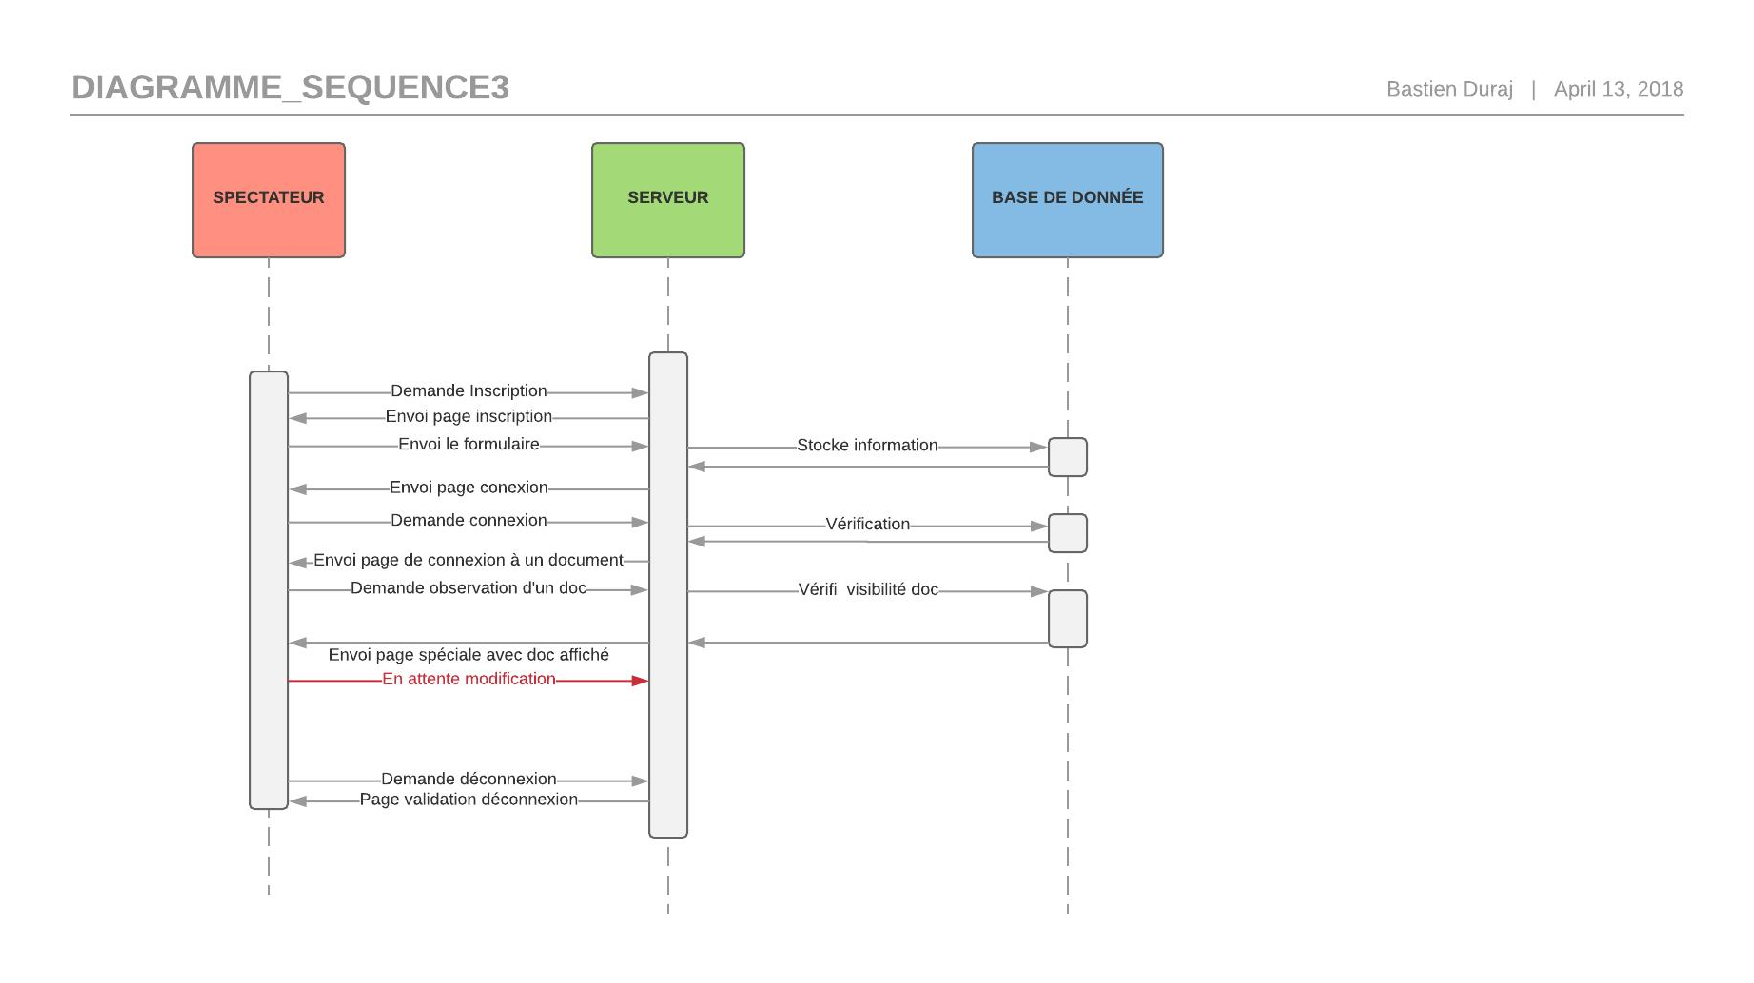
\includegraphics[scale=0.7]{Image/Diagramme_sequence3.pdf}
\caption{Représente le déroulement d'un scénario entre trois acteurs: Spectateur, serveur, BDD}
\end{figure}
\subsection{Diagramme des classes}
\newpage
\begin{figure}[!h]
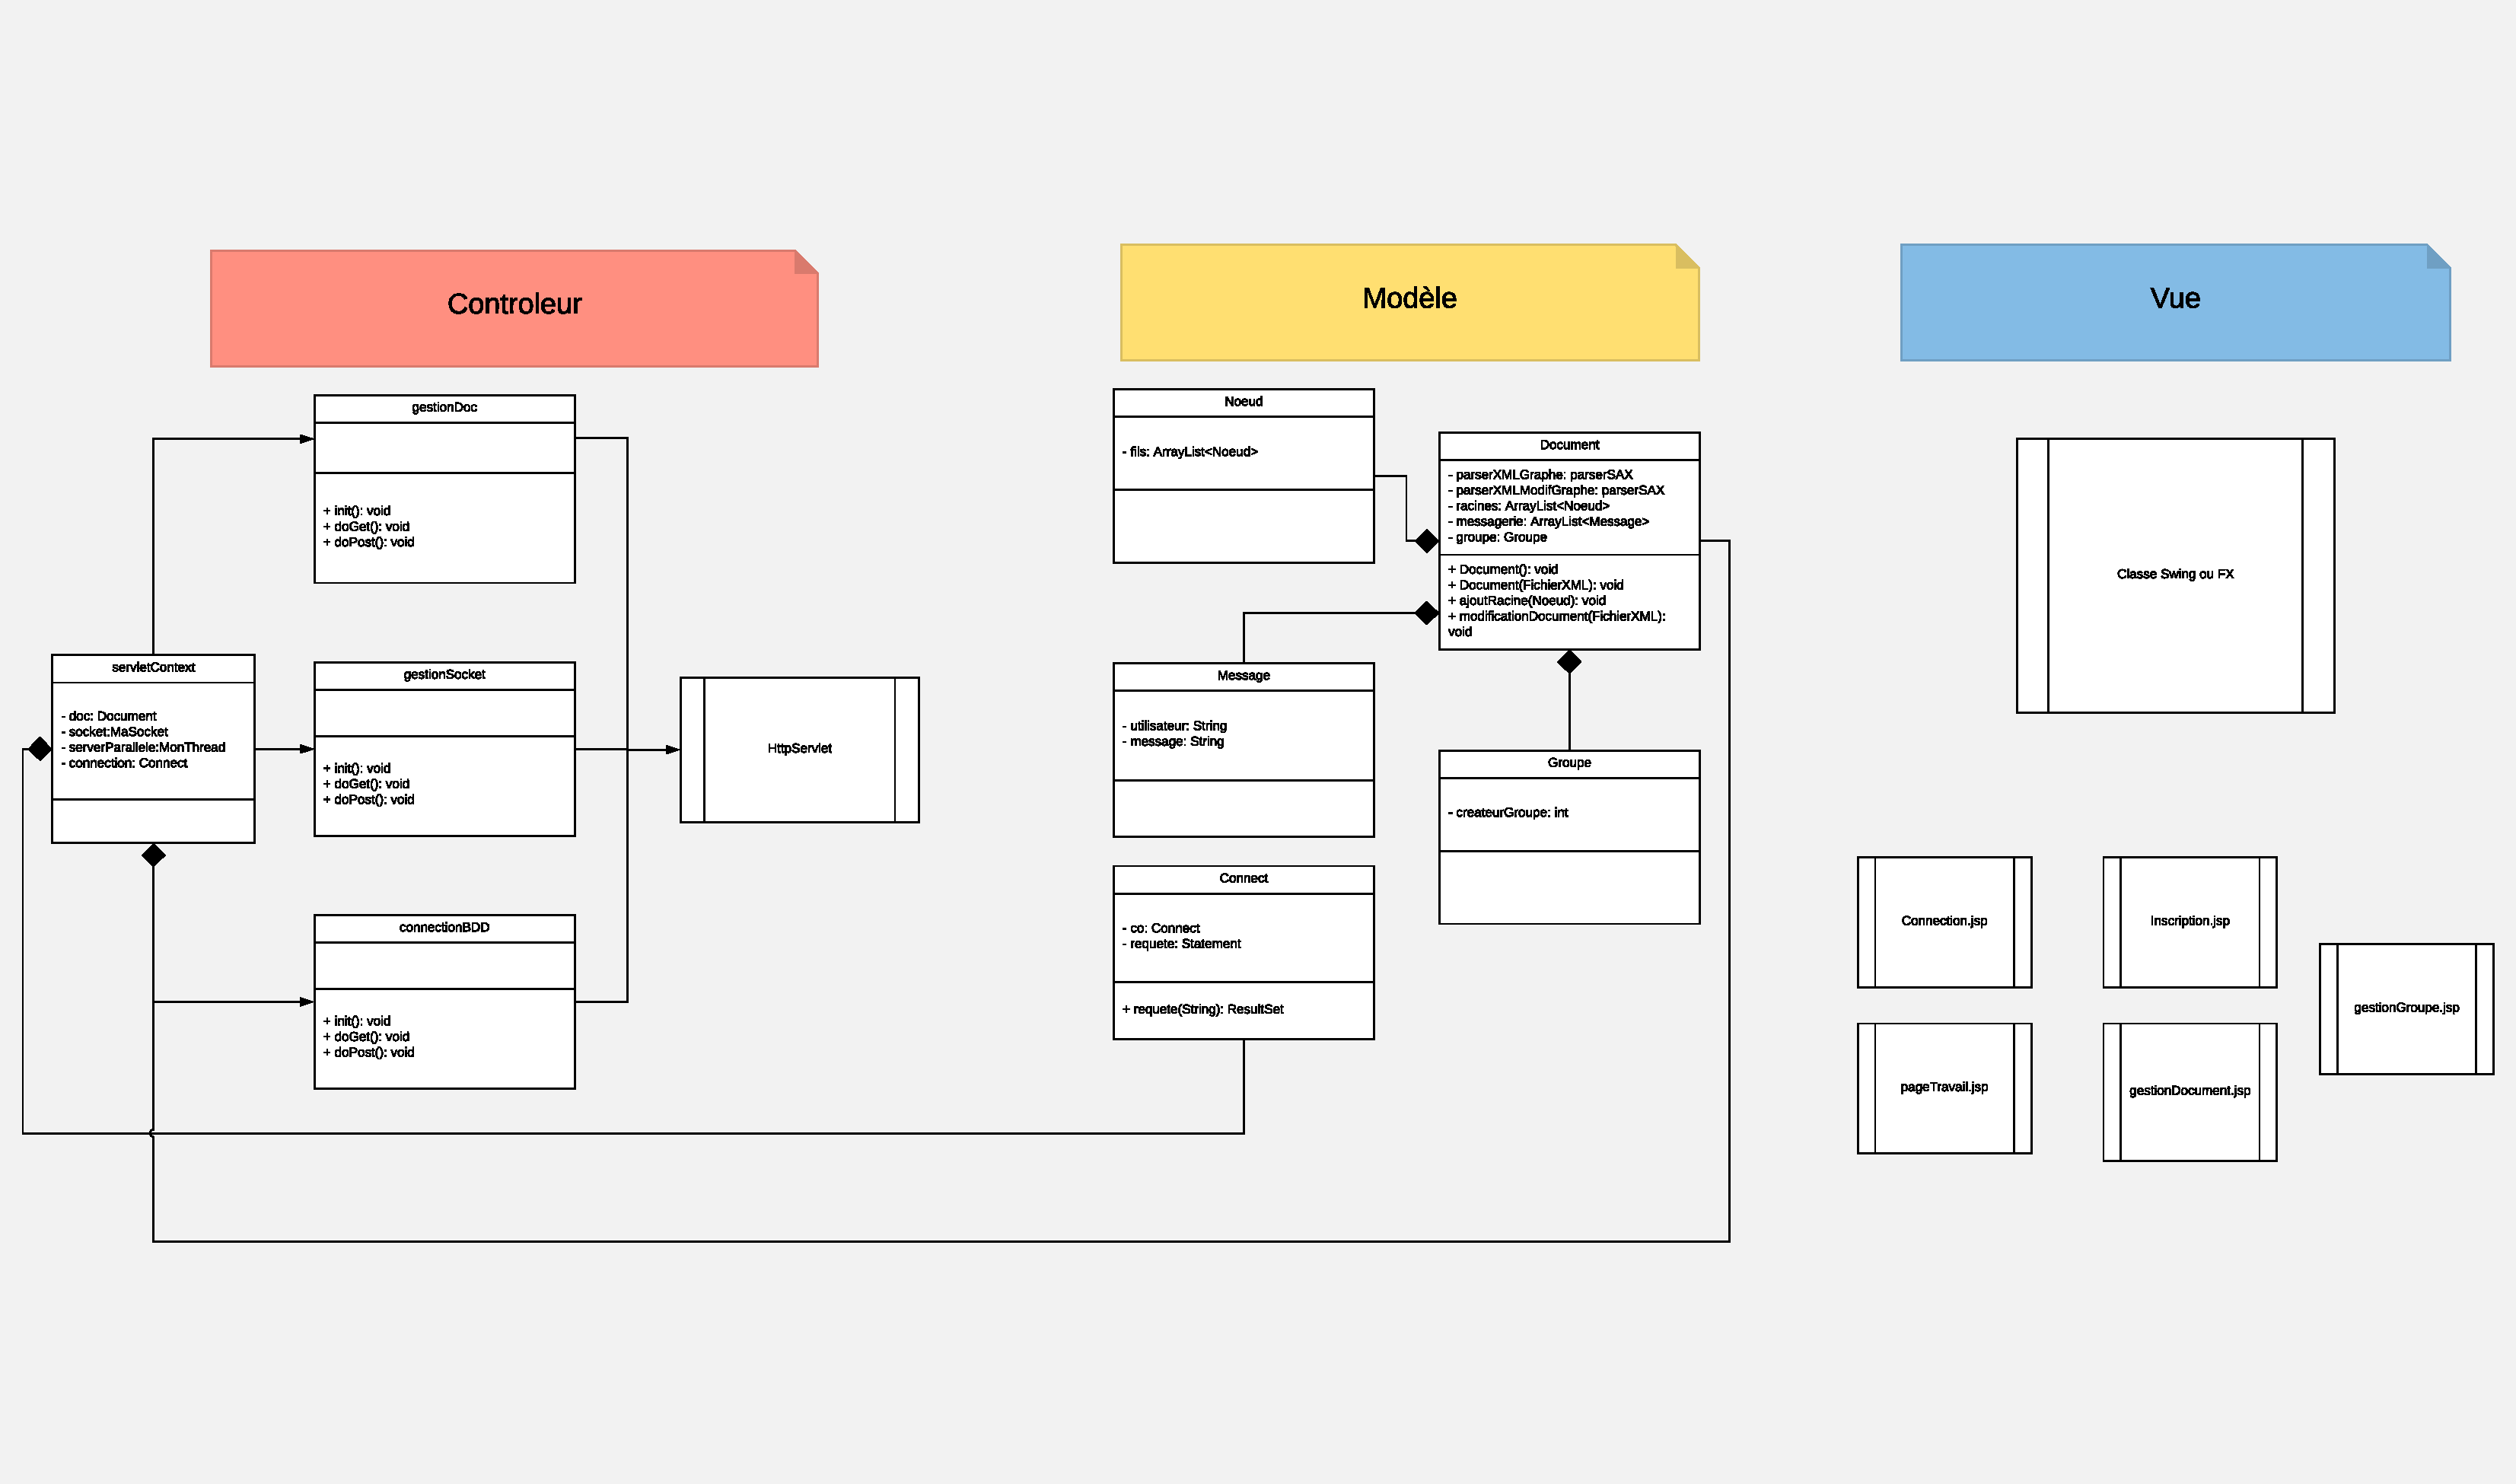
\includegraphics[angle=270, scale=0.4]{Image/Class_Diagram_dev2.pdf}
\caption{Diagramme des classes de notre application divisé en 3 parties suivant l'architecture MVC pour plus de visibilité}
\end{figure}

\end{document}
